\begin{enumerate}[label=\thesubsection.\arabic*.,ref=\thesubsection.\theenumi]
\numberwithin{equation}{enumi}
\item Using the frequency response method, design a lag-lead compensator for the unity feedback system given 
\begin{align}
G(S) = \frac{K(s+7)}{s(s+5)(s+15)}
\end{align}
The following specifications must be met: Peak overshoot = 15\%, settling time = 0.1 second and velocity error constant = 1000
Use second order approximation. \\
%
\solution Figure: \ref{fig:1;} models the equivalent of compensated closed loop system. 
\begin{figure}[!ht]
\begin{center}
		\resizebox{\columnwidth}{!}{\begin{enumerate}[label=\thesubsection.\arabic*.,ref=\thesubsection.\theenumi]
\numberwithin{equation}{enumi}
\item Using the frequency response method, design a lag-lead compensator for the unity feedback system given 
\begin{align}
G(S) = \frac{K(s+7)}{s(s+5)(s+15)}
\end{align}
The following specifications must be met: Peak overshoot = 15\%, settling time = 0.1 second and velocity error constant = 1000
Use second order approximation. \\
%
\solution Figure: \ref{fig:1;} models the equivalent of compensated closed loop system. 
\begin{figure}[!ht]
\begin{center}
		\resizebox{\columnwidth}{!}{\begin{enumerate}[label=\thesubsection.\arabic*.,ref=\thesubsection.\theenumi]
\numberwithin{equation}{enumi}
\item Using the frequency response method, design a lag-lead compensator for the unity feedback system given 
\begin{align}
G(S) = \frac{K(s+7)}{s(s+5)(s+15)}
\end{align}
The following specifications must be met: Peak overshoot = 15\%, settling time = 0.1 second and velocity error constant = 1000
Use second order approximation. \\
%
\solution Figure: \ref{fig:1;} models the equivalent of compensated closed loop system. 
\begin{figure}[!ht]
\begin{center}
		\resizebox{\columnwidth}{!}{\begin{enumerate}[label=\thesubsection.\arabic*.,ref=\thesubsection.\theenumi]
\numberwithin{equation}{enumi}
\item Using the frequency response method, design a lag-lead compensator for the unity feedback system given 
\begin{align}
G(S) = \frac{K(s+7)}{s(s+5)(s+15)}
\end{align}
The following specifications must be met: Peak overshoot = 15\%, settling time = 0.1 second and velocity error constant = 1000
Use second order approximation. \\
%
\solution Figure: \ref{fig:1;} models the equivalent of compensated closed loop system. 
\begin{figure}[!ht]
\begin{center}
		\resizebox{\columnwidth}{!}{\input{./figs/ee18btech11012/ee18btech11012_1.tex}}
\end{center}
\caption{}
\label{fig:ee18btech11012_1;}
\end{figure}
%
Velocity error constant  
\begin{align}
K_{v} &=  \lim_{s \to 0}sG(s)
\end{align}
\begin{align}
\lim_{s \to 0}s\frac{K(s+7)}{s(s+5)(s+15)} &= 1000
\end{align}
\begin{align}
\implies K &= 10714
\end{align}
Bode plot of G(s) for the value of K
%%
\begin{figure}[!ht]
\centering
  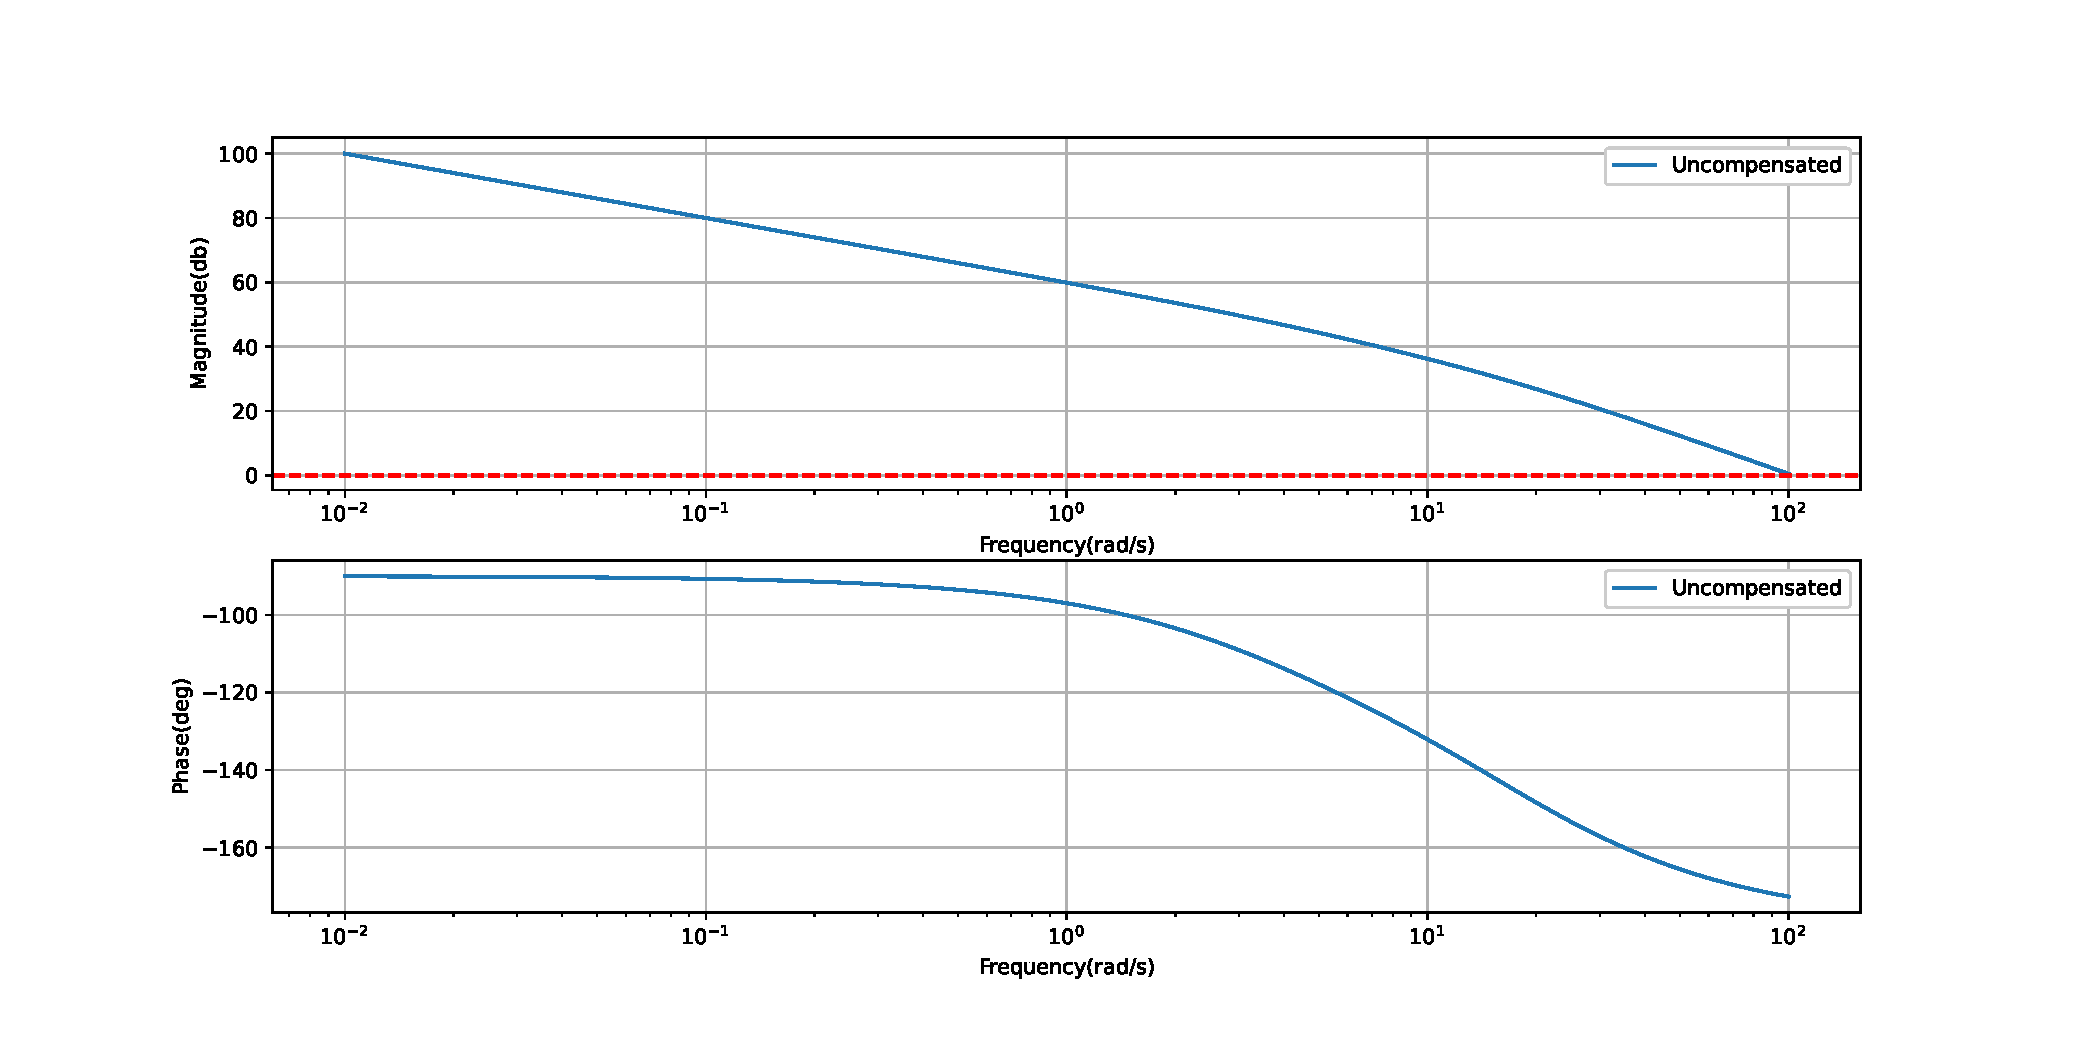
\includegraphics[width=\columnwidth]{./figs/ee18btech11012/ee18btech11012.eps}
\caption{}
\label{fig:ee18btech11012_2}
\end{figure}
%%
The following code verifies the result.
\begin{lstlisting}
codes/ee18btech11012/ee18btech11012_1.py
\end{lstlisting}
Relation between \%OS and Damping ratio
\begin{align}
\zeta &= \frac{-\ln(\%OS/100)}{\sqrt{(\pi)^2 + (\ln(\%OS/100))^2}}
\end{align}
\begin{align}
\implies\zeta &= 0.517 
\end{align}
Phase Margin for a Damping ratio is given by
\begin{align}
\phi_{m} &= 90\degree - \arctan(\frac{\sqrt{-2\zeta^2+\sqrt{1+4\zeta^4}}}{2\zeta}
\end{align}
\begin{align}
\implies \phi_{m} &= 53.17\degree
\end{align}
For an additional 5\degree for lag compensation,Phase margin is
\begin{align}
    \phi_{m} &= 53.17\degree + 5\degree= 58.17\degree
\end{align}
\textbf{Note} : Adding 5\degree phase angle to compensate the phase angle contribution of the lag compensator.
Bandwidth frequency is given by
\begin{align}
\omega_{BW} &= \omega_{n}(\sqrt{(1-2\zeta^2)+\sqrt{4\zeta^4-4\zeta^2+2}})
\end{align}
where
\begin{align}
    \omega_{n} &= \frac{4}{T_{s}\zeta}
\end{align}
Given settling time = 0.1 sec then 
\begin{align}
    \omega_{n} &= 77.37 rad/sec 
\end{align}
then
\begin{align}
    \omega_{BW} &= 96.91 rad/sec
\end{align}
\item Designing Lag-Lead Compensator Gc(s) \\
\solution 
General lag-lead compensator 
\begin{align}
G_{c}(s) &= \left(\frac{s+\frac{1}{T_1}}{s+\frac{\gamma}{T_1}}\right)\left(\frac{s+\frac{1}{T_2}}{s+\frac{1}{\gamma T_2}}\right) 
\end{align}
\begin{itemize}
\item Choose the new phase-margin frequency 
\begin{align}
    \omega_{Pm} &= 0.8 \omega_{BW} &= 77.53 rad/sec
\end{align}
\item At this phase-margin frequency,Phase angle is -170.52\degree.
\item Then the conribution required from the lead is
\begin{align}
    \phi_{max} &= 58.17-(180-170.52)=48.69\degree.
\end{align}

\item Now Using the relation 
\begin{align}
    \phi_{max} &= \sin^{-1}(\frac{1-\beta}{1+\beta})
\end{align}
then we get
\begin{align}
    \beta &= 0.142
\end{align}
\item \underline{Lag Compensator Design}:The Compensator must have a dc gain of unity to retain the value of Kv that we have already designed by setting K = 10714.
\begin{align}
    z_{clag} &= \frac{\omega_{Pm}}{10}=\frac{77.53}{10}=7.753
\end{align}
\begin{align}
    p_{clag} &= z_{clag}*\beta=1.102
\end{align}
Gain in the lag compensator is 
\begin{align}
    K_{clag} &= \frac{p_{clag}}{z_{clag}}=0.1421
\end{align}
\item Hence the lag compensator transfer function is
\begin{align}
 G_{clag}(s) &= \frac{0.1421(s+7.753)}{s+1.102} 
\end{align}
\item \underline{Lead Compensator Design}:DC gain for this must be unity.

\textbf{Relations to find T and $\beta$}:
The Compensator's magnitude at the phase margin frequency $\omega_{max}$
\begin{align}
     |G_{c}(j\omega_{max})| &= \frac{1}{\sqrt{\beta}} 
\end{align}
\begin{align}
    T &= \frac{1}{\omega_{max}\sqrt{\beta}}
\end{align}
So,To find transfer function
\begin{align}
    z_{lead} &= \frac{1}{T_{2}}=\omega_{Pm}*\sqrt{\beta}=29.92
\end{align}
\begin{align}
    p_{lead} &= \frac{z_{lead}}{\beta}=205.74,K_{lead}=\frac{p_{lead}}{z_{lead}}=7.04
\end{align}
\item Thus lead compensator transfer function is 
\begin{align}
    G_{lead} &= \frac{7.04(s+29.22)}{s+205.74} 
\end{align}
\item So the overall compensator tranfer function is
\begin{align}
    G_{c}(s) &= G_{clag}(s)G_{lead}(s)
\end{align}
\begin{align}
G_{c}(s)&=\frac{1.000384(s+7.753)(s+29.23)}{(s+1.102)(s+205.7)}
\end{align}
\end{itemize}
\item Verifying Lag-lead Compensator using Plots \\
\solution 
Magnitude and Phase plot
\begin{figure}[!ht]
\centering
  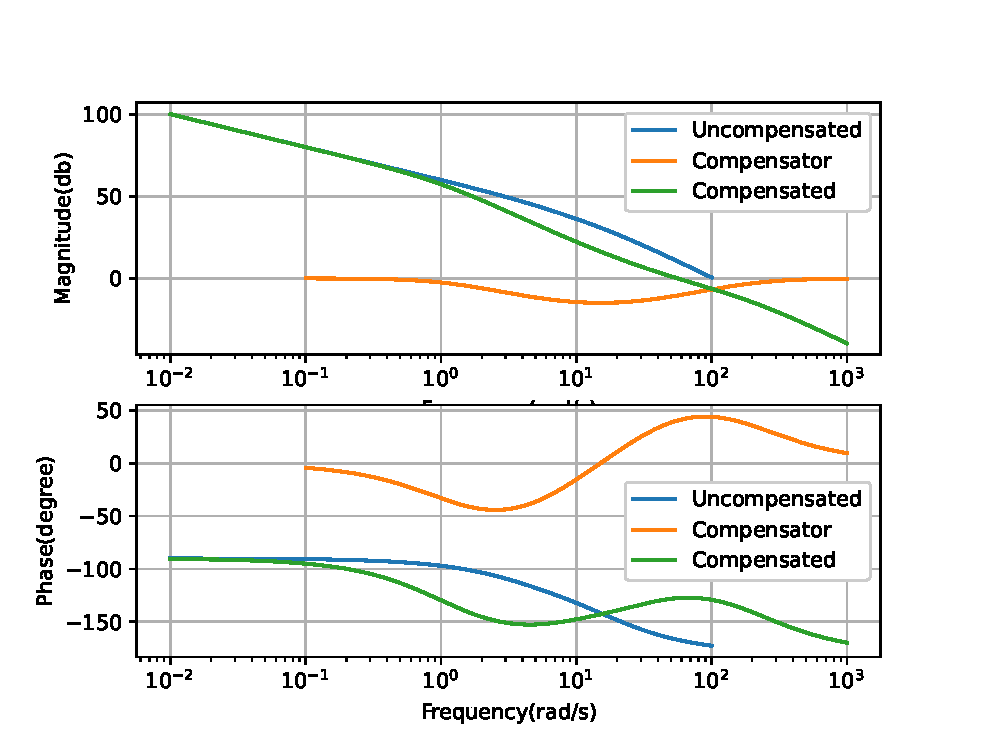
\includegraphics[width=\columnwidth]{./figs/ee18btech11012/ee18btech11012_2.eps}
\caption{}
\label{fig:ee18btech11012_3}
\end{figure}
The following code 
\begin{lstlisting}
codes/ee18btech11012/ee18btech11012_2.py
\end{lstlisting}
\item Verifying in time domain \\
\solution 
Time response for a unit step function
\begin{figure}[!ht]
\centering
  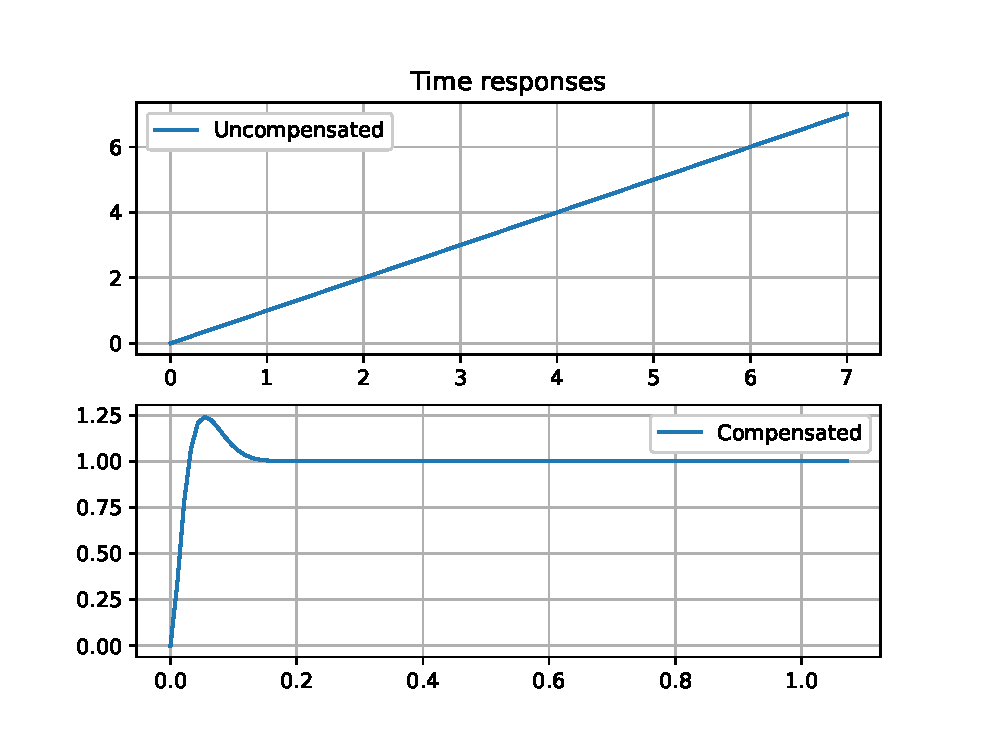
\includegraphics[width=\columnwidth]{./figs/ee18btech11012/ee18btech11012_3.eps}
\caption{}
\label{fig:ee18btech11012_4} 
\end{figure}
The following code can be verified
\begin{lstlisting}
codes/ee18btech11012/ee18btech11012_3.py
\end{lstlisting}
\item Verifying the designed lag-lead compensator \\
\solution 
\begin{table}[!ht]
\centering
\input{./tables/ee18btech11012/ee18btech11012_table1.tex}
\caption{Comparing the desired and obtained results}
\label{table:ee18btech11012_table1}
\end{table}
\end{enumerate}
}
\end{center}
\caption{}
\label{fig:ee18btech11012_1;}
\end{figure}
%
Velocity error constant  
\begin{align}
K_{v} &=  \lim_{s \to 0}sG(s)
\end{align}
\begin{align}
\lim_{s \to 0}s\frac{K(s+7)}{s(s+5)(s+15)} &= 1000
\end{align}
\begin{align}
\implies K &= 10714
\end{align}
Bode plot of G(s) for the value of K
%%
\begin{figure}[!ht]
\centering
  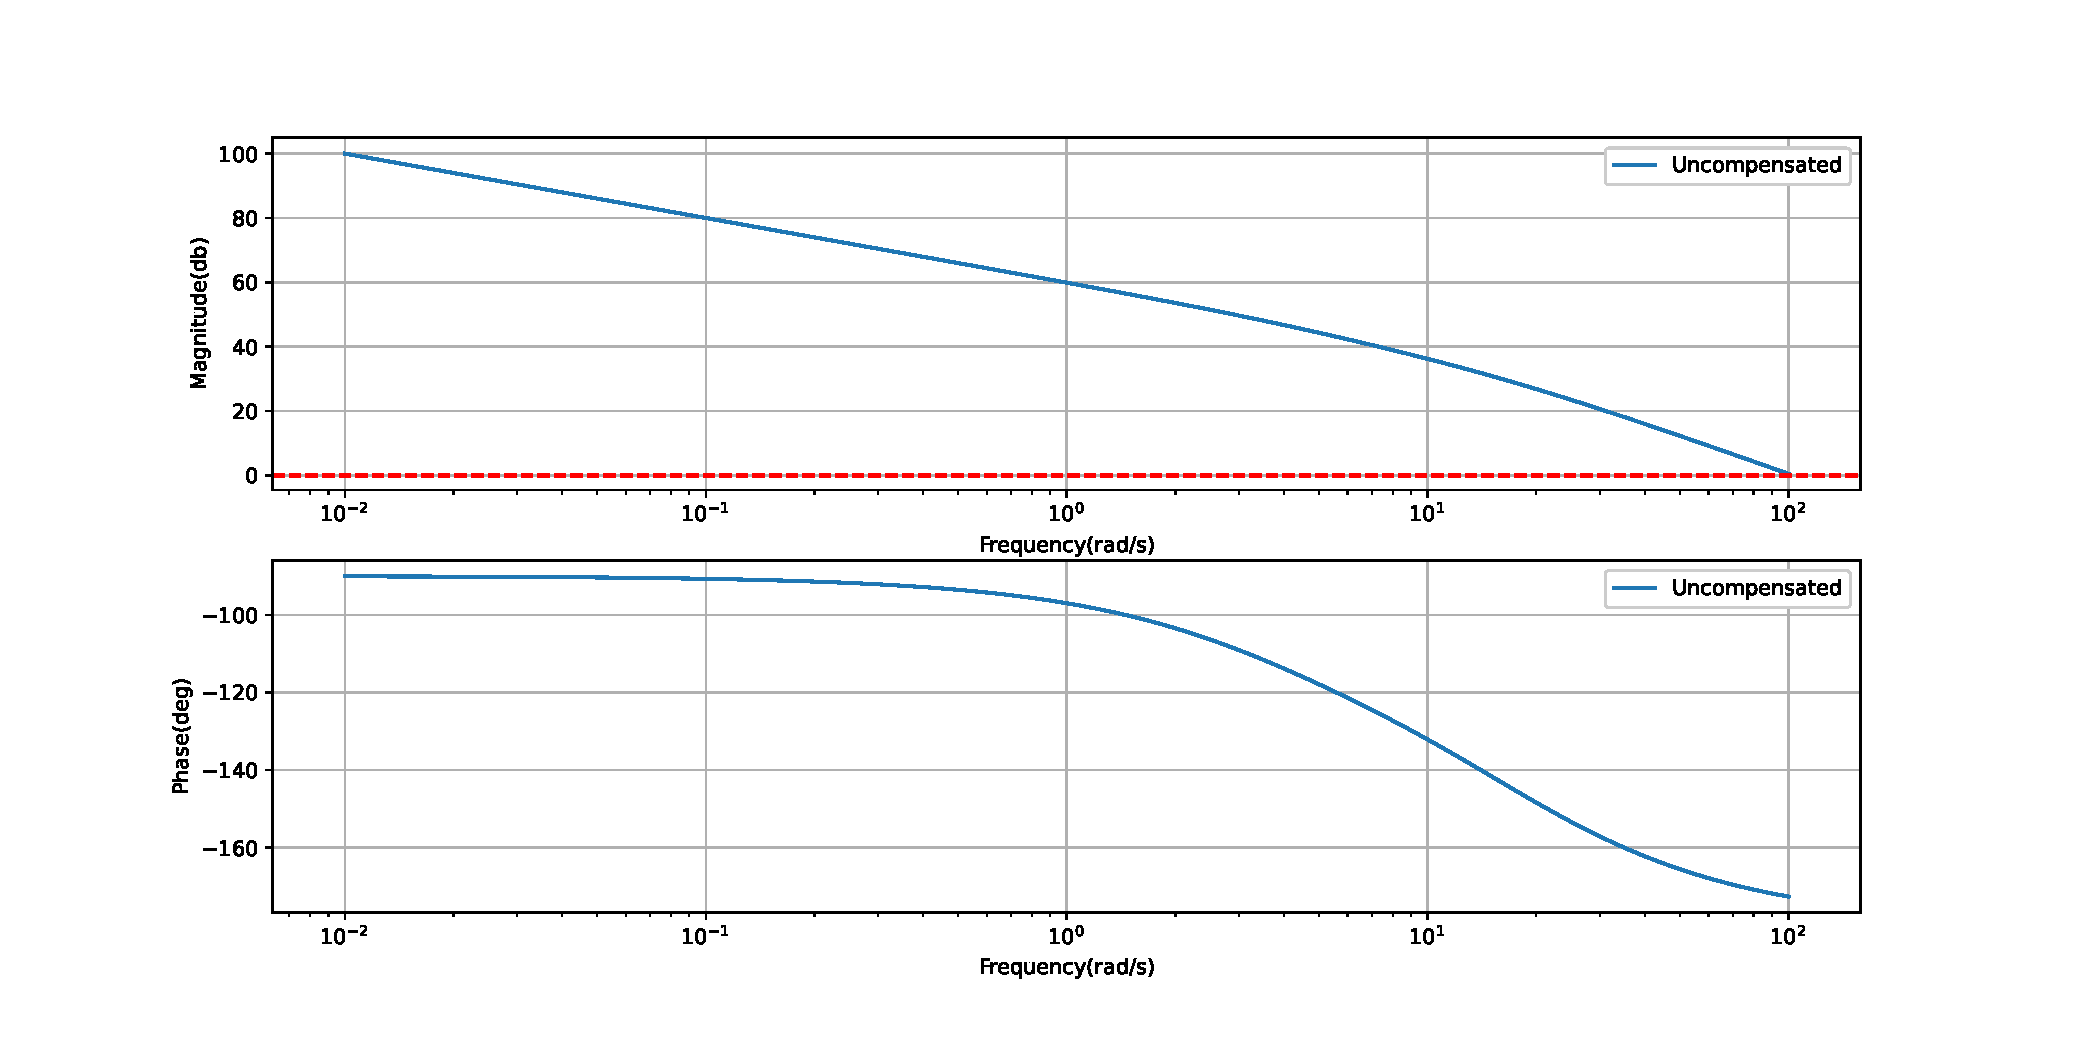
\includegraphics[width=\columnwidth]{./figs/ee18btech11012/ee18btech11012.eps}
\caption{}
\label{fig:ee18btech11012_2}
\end{figure}
%%
The following code verifies the result.
\begin{lstlisting}
codes/ee18btech11012/ee18btech11012_1.py
\end{lstlisting}
Relation between \%OS and Damping ratio
\begin{align}
\zeta &= \frac{-\ln(\%OS/100)}{\sqrt{(\pi)^2 + (\ln(\%OS/100))^2}}
\end{align}
\begin{align}
\implies\zeta &= 0.517 
\end{align}
Phase Margin for a Damping ratio is given by
\begin{align}
\phi_{m} &= 90\degree - \arctan(\frac{\sqrt{-2\zeta^2+\sqrt{1+4\zeta^4}}}{2\zeta}
\end{align}
\begin{align}
\implies \phi_{m} &= 53.17\degree
\end{align}
For an additional 5\degree for lag compensation,Phase margin is
\begin{align}
    \phi_{m} &= 53.17\degree + 5\degree= 58.17\degree
\end{align}
\textbf{Note} : Adding 5\degree phase angle to compensate the phase angle contribution of the lag compensator.
Bandwidth frequency is given by
\begin{align}
\omega_{BW} &= \omega_{n}(\sqrt{(1-2\zeta^2)+\sqrt{4\zeta^4-4\zeta^2+2}})
\end{align}
where
\begin{align}
    \omega_{n} &= \frac{4}{T_{s}\zeta}
\end{align}
Given settling time = 0.1 sec then 
\begin{align}
    \omega_{n} &= 77.37 rad/sec 
\end{align}
then
\begin{align}
    \omega_{BW} &= 96.91 rad/sec
\end{align}
\item Designing Lag-Lead Compensator Gc(s) \\
\solution 
General lag-lead compensator 
\begin{align}
G_{c}(s) &= \left(\frac{s+\frac{1}{T_1}}{s+\frac{\gamma}{T_1}}\right)\left(\frac{s+\frac{1}{T_2}}{s+\frac{1}{\gamma T_2}}\right) 
\end{align}
\begin{itemize}
\item Choose the new phase-margin frequency 
\begin{align}
    \omega_{Pm} &= 0.8 \omega_{BW} &= 77.53 rad/sec
\end{align}
\item At this phase-margin frequency,Phase angle is -170.52\degree.
\item Then the conribution required from the lead is
\begin{align}
    \phi_{max} &= 58.17-(180-170.52)=48.69\degree.
\end{align}

\item Now Using the relation 
\begin{align}
    \phi_{max} &= \sin^{-1}(\frac{1-\beta}{1+\beta})
\end{align}
then we get
\begin{align}
    \beta &= 0.142
\end{align}
\item \underline{Lag Compensator Design}:The Compensator must have a dc gain of unity to retain the value of Kv that we have already designed by setting K = 10714.
\begin{align}
    z_{clag} &= \frac{\omega_{Pm}}{10}=\frac{77.53}{10}=7.753
\end{align}
\begin{align}
    p_{clag} &= z_{clag}*\beta=1.102
\end{align}
Gain in the lag compensator is 
\begin{align}
    K_{clag} &= \frac{p_{clag}}{z_{clag}}=0.1421
\end{align}
\item Hence the lag compensator transfer function is
\begin{align}
 G_{clag}(s) &= \frac{0.1421(s+7.753)}{s+1.102} 
\end{align}
\item \underline{Lead Compensator Design}:DC gain for this must be unity.

\textbf{Relations to find T and $\beta$}:
The Compensator's magnitude at the phase margin frequency $\omega_{max}$
\begin{align}
     |G_{c}(j\omega_{max})| &= \frac{1}{\sqrt{\beta}} 
\end{align}
\begin{align}
    T &= \frac{1}{\omega_{max}\sqrt{\beta}}
\end{align}
So,To find transfer function
\begin{align}
    z_{lead} &= \frac{1}{T_{2}}=\omega_{Pm}*\sqrt{\beta}=29.92
\end{align}
\begin{align}
    p_{lead} &= \frac{z_{lead}}{\beta}=205.74,K_{lead}=\frac{p_{lead}}{z_{lead}}=7.04
\end{align}
\item Thus lead compensator transfer function is 
\begin{align}
    G_{lead} &= \frac{7.04(s+29.22)}{s+205.74} 
\end{align}
\item So the overall compensator tranfer function is
\begin{align}
    G_{c}(s) &= G_{clag}(s)G_{lead}(s)
\end{align}
\begin{align}
G_{c}(s)&=\frac{1.000384(s+7.753)(s+29.23)}{(s+1.102)(s+205.7)}
\end{align}
\end{itemize}
\item Verifying Lag-lead Compensator using Plots \\
\solution 
Magnitude and Phase plot
\begin{figure}[!ht]
\centering
  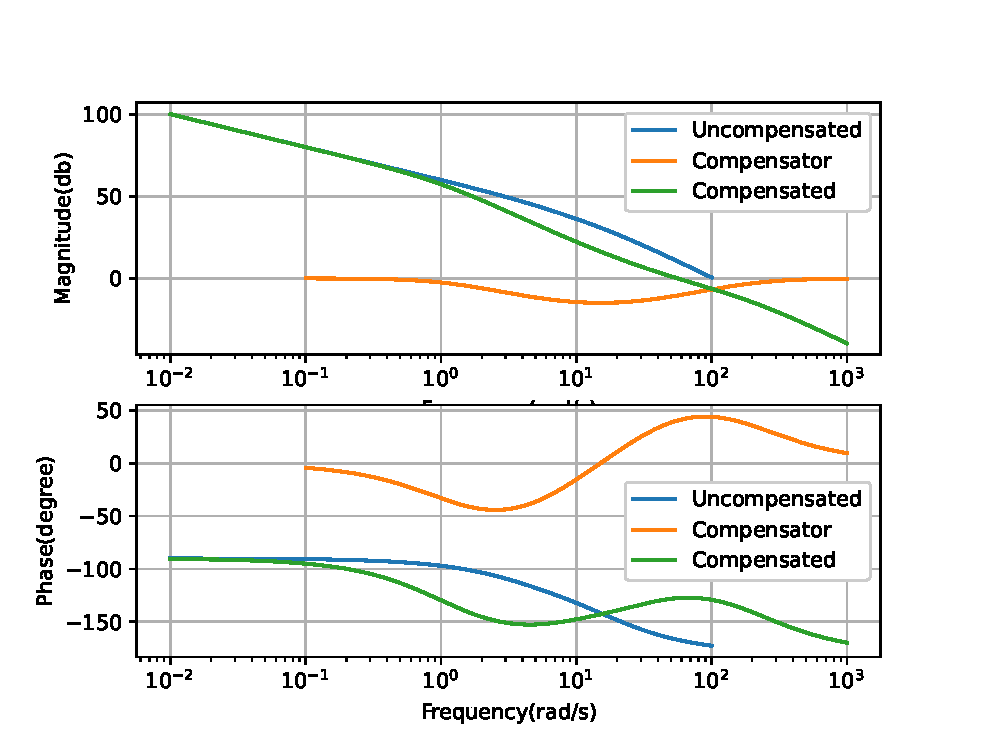
\includegraphics[width=\columnwidth]{./figs/ee18btech11012/ee18btech11012_2.eps}
\caption{}
\label{fig:ee18btech11012_3}
\end{figure}
The following code 
\begin{lstlisting}
codes/ee18btech11012/ee18btech11012_2.py
\end{lstlisting}
\item Verifying in time domain \\
\solution 
Time response for a unit step function
\begin{figure}[!ht]
\centering
  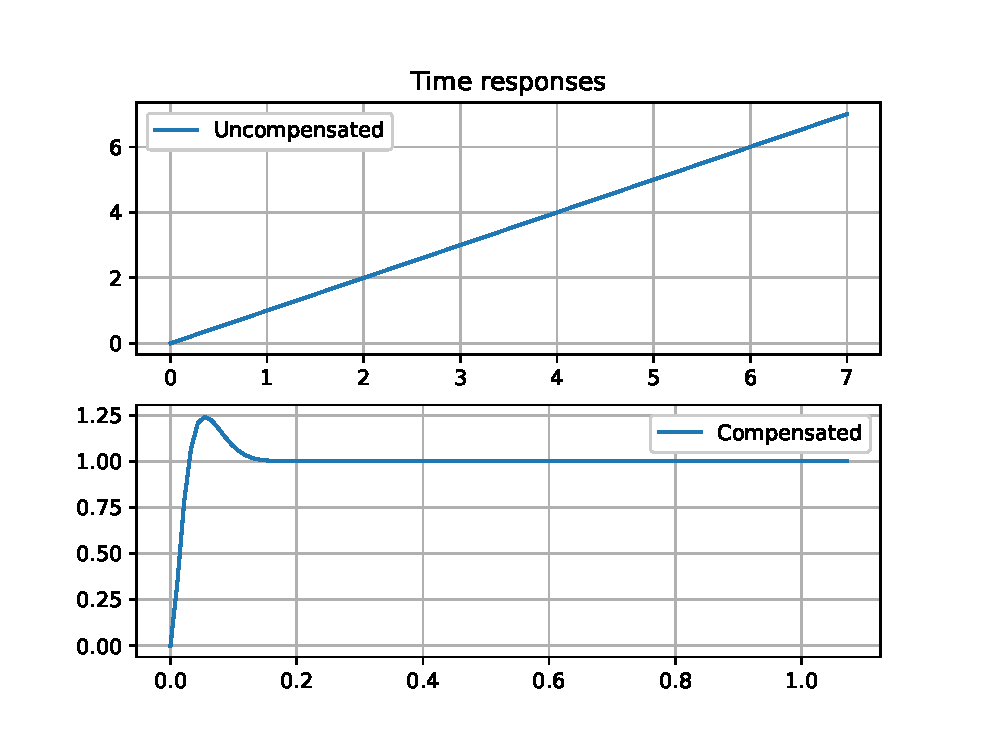
\includegraphics[width=\columnwidth]{./figs/ee18btech11012/ee18btech11012_3.eps}
\caption{}
\label{fig:ee18btech11012_4} 
\end{figure}
The following code can be verified
\begin{lstlisting}
codes/ee18btech11012/ee18btech11012_3.py
\end{lstlisting}
\item Verifying the designed lag-lead compensator \\
\solution 
\begin{table}[!ht]
\centering
\input{./tables/ee18btech11012/ee18btech11012_table1.tex}
\caption{Comparing the desired and obtained results}
\label{table:ee18btech11012_table1}
\end{table}
\end{enumerate}
}
\end{center}
\caption{}
\label{fig:ee18btech11012_1;}
\end{figure}
%
Velocity error constant  
\begin{align}
K_{v} &=  \lim_{s \to 0}sG(s)
\end{align}
\begin{align}
\lim_{s \to 0}s\frac{K(s+7)}{s(s+5)(s+15)} &= 1000
\end{align}
\begin{align}
\implies K &= 10714
\end{align}
Bode plot of G(s) for the value of K
%%
\begin{figure}[!ht]
\centering
  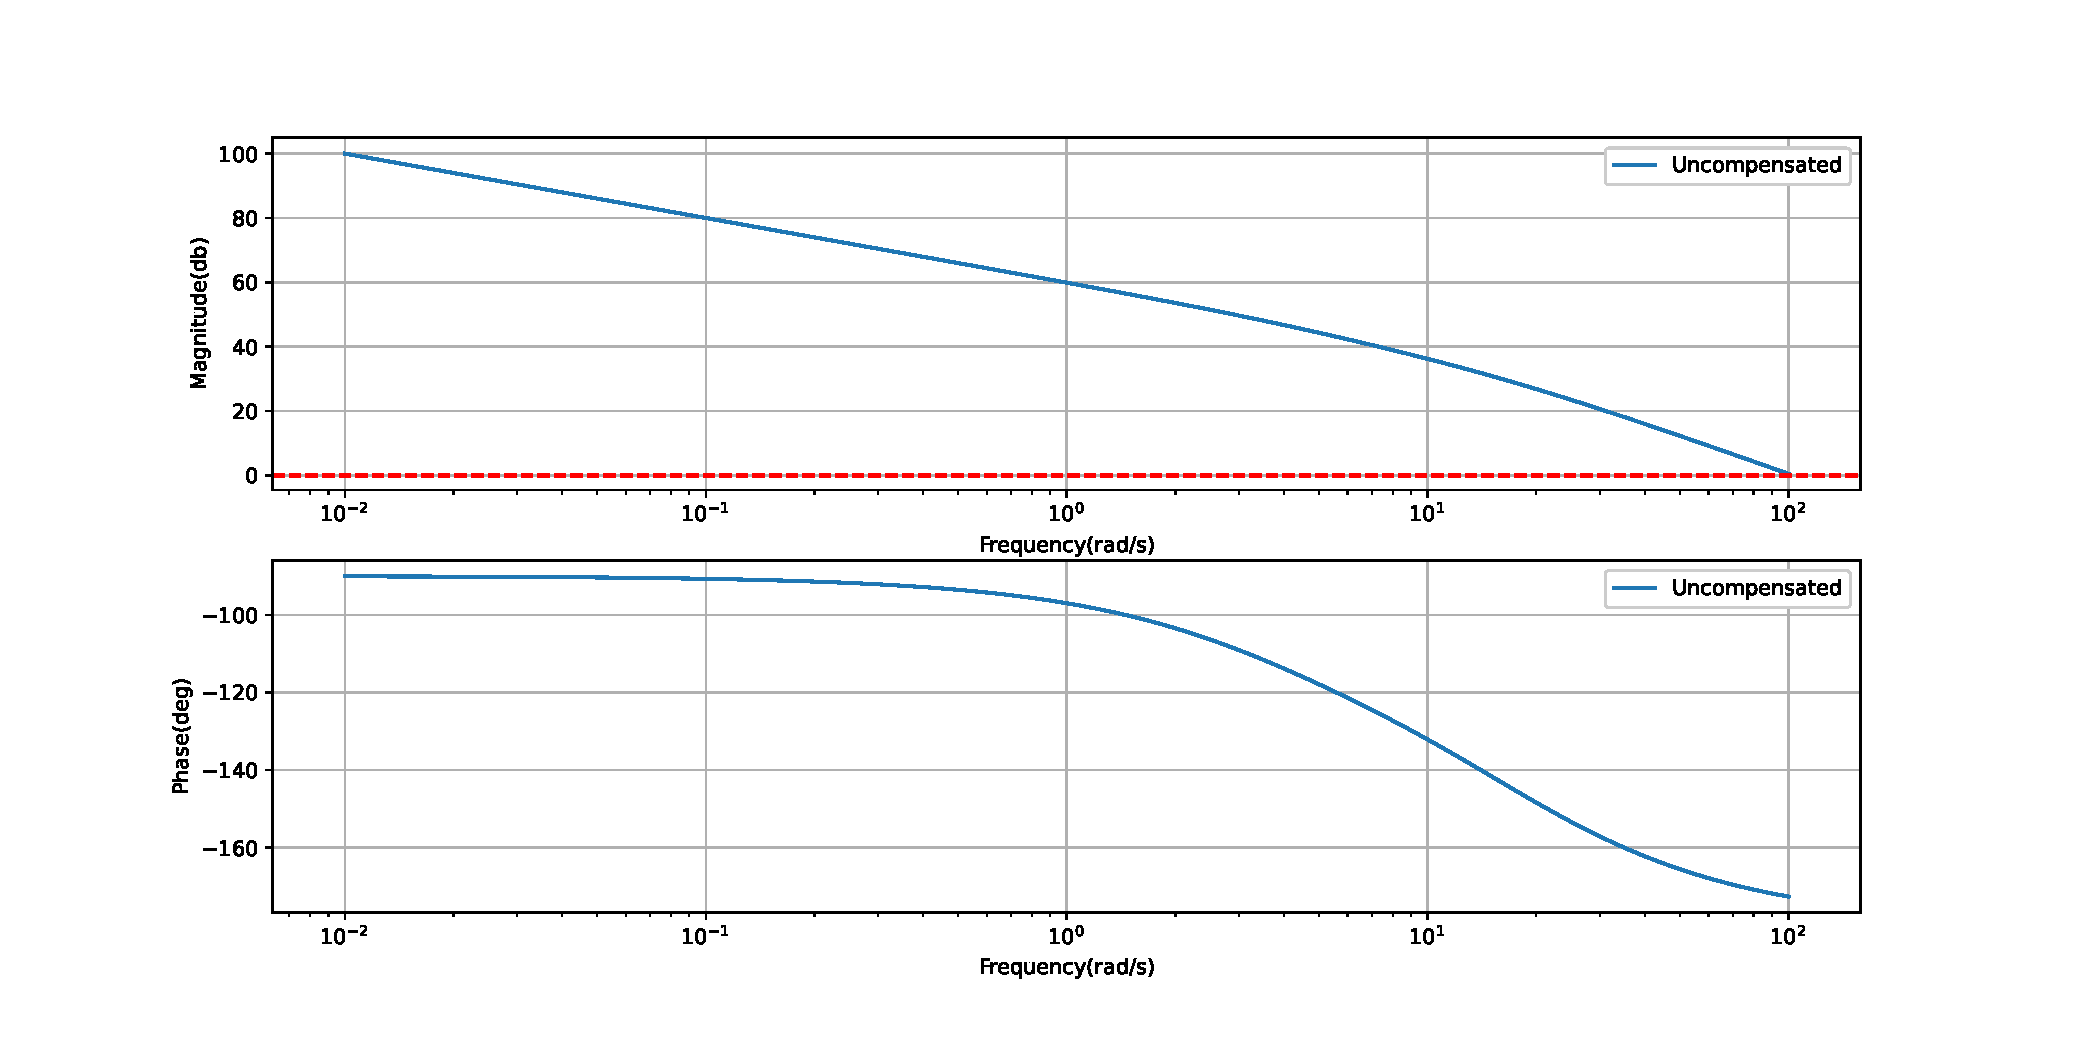
\includegraphics[width=\columnwidth]{./figs/ee18btech11012/ee18btech11012.eps}
\caption{}
\label{fig:ee18btech11012_2}
\end{figure}
%%
The following code verifies the result.
\begin{lstlisting}
codes/ee18btech11012/ee18btech11012_1.py
\end{lstlisting}
Relation between \%OS and Damping ratio
\begin{align}
\zeta &= \frac{-\ln(\%OS/100)}{\sqrt{(\pi)^2 + (\ln(\%OS/100))^2}}
\end{align}
\begin{align}
\implies\zeta &= 0.517 
\end{align}
Phase Margin for a Damping ratio is given by
\begin{align}
\phi_{m} &= 90\degree - \arctan(\frac{\sqrt{-2\zeta^2+\sqrt{1+4\zeta^4}}}{2\zeta}
\end{align}
\begin{align}
\implies \phi_{m} &= 53.17\degree
\end{align}
For an additional 5\degree for lag compensation,Phase margin is
\begin{align}
    \phi_{m} &= 53.17\degree + 5\degree= 58.17\degree
\end{align}
\textbf{Note} : Adding 5\degree phase angle to compensate the phase angle contribution of the lag compensator.
Bandwidth frequency is given by
\begin{align}
\omega_{BW} &= \omega_{n}(\sqrt{(1-2\zeta^2)+\sqrt{4\zeta^4-4\zeta^2+2}})
\end{align}
where
\begin{align}
    \omega_{n} &= \frac{4}{T_{s}\zeta}
\end{align}
Given settling time = 0.1 sec then 
\begin{align}
    \omega_{n} &= 77.37 rad/sec 
\end{align}
then
\begin{align}
    \omega_{BW} &= 96.91 rad/sec
\end{align}
\item Designing Lag-Lead Compensator Gc(s) \\
\solution 
General lag-lead compensator 
\begin{align}
G_{c}(s) &= \left(\frac{s+\frac{1}{T_1}}{s+\frac{\gamma}{T_1}}\right)\left(\frac{s+\frac{1}{T_2}}{s+\frac{1}{\gamma T_2}}\right) 
\end{align}
\begin{itemize}
\item Choose the new phase-margin frequency 
\begin{align}
    \omega_{Pm} &= 0.8 \omega_{BW} &= 77.53 rad/sec
\end{align}
\item At this phase-margin frequency,Phase angle is -170.52\degree.
\item Then the conribution required from the lead is
\begin{align}
    \phi_{max} &= 58.17-(180-170.52)=48.69\degree.
\end{align}

\item Now Using the relation 
\begin{align}
    \phi_{max} &= \sin^{-1}(\frac{1-\beta}{1+\beta})
\end{align}
then we get
\begin{align}
    \beta &= 0.142
\end{align}
\item \underline{Lag Compensator Design}:The Compensator must have a dc gain of unity to retain the value of Kv that we have already designed by setting K = 10714.
\begin{align}
    z_{clag} &= \frac{\omega_{Pm}}{10}=\frac{77.53}{10}=7.753
\end{align}
\begin{align}
    p_{clag} &= z_{clag}*\beta=1.102
\end{align}
Gain in the lag compensator is 
\begin{align}
    K_{clag} &= \frac{p_{clag}}{z_{clag}}=0.1421
\end{align}
\item Hence the lag compensator transfer function is
\begin{align}
 G_{clag}(s) &= \frac{0.1421(s+7.753)}{s+1.102} 
\end{align}
\item \underline{Lead Compensator Design}:DC gain for this must be unity.

\textbf{Relations to find T and $\beta$}:
The Compensator's magnitude at the phase margin frequency $\omega_{max}$
\begin{align}
     |G_{c}(j\omega_{max})| &= \frac{1}{\sqrt{\beta}} 
\end{align}
\begin{align}
    T &= \frac{1}{\omega_{max}\sqrt{\beta}}
\end{align}
So,To find transfer function
\begin{align}
    z_{lead} &= \frac{1}{T_{2}}=\omega_{Pm}*\sqrt{\beta}=29.92
\end{align}
\begin{align}
    p_{lead} &= \frac{z_{lead}}{\beta}=205.74,K_{lead}=\frac{p_{lead}}{z_{lead}}=7.04
\end{align}
\item Thus lead compensator transfer function is 
\begin{align}
    G_{lead} &= \frac{7.04(s+29.22)}{s+205.74} 
\end{align}
\item So the overall compensator tranfer function is
\begin{align}
    G_{c}(s) &= G_{clag}(s)G_{lead}(s)
\end{align}
\begin{align}
G_{c}(s)&=\frac{1.000384(s+7.753)(s+29.23)}{(s+1.102)(s+205.7)}
\end{align}
\end{itemize}
\item Verifying Lag-lead Compensator using Plots \\
\solution 
Magnitude and Phase plot
\begin{figure}[!ht]
\centering
  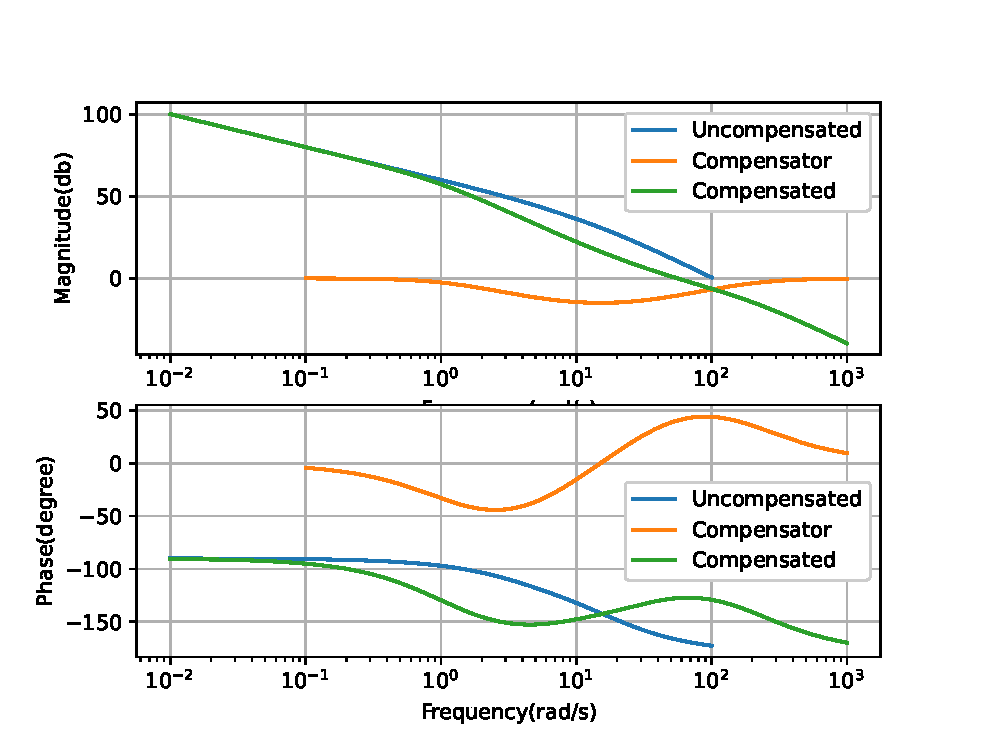
\includegraphics[width=\columnwidth]{./figs/ee18btech11012/ee18btech11012_2.eps}
\caption{}
\label{fig:ee18btech11012_3}
\end{figure}
The following code 
\begin{lstlisting}
codes/ee18btech11012/ee18btech11012_2.py
\end{lstlisting}
\item Verifying in time domain \\
\solution 
Time response for a unit step function
\begin{figure}[!ht]
\centering
  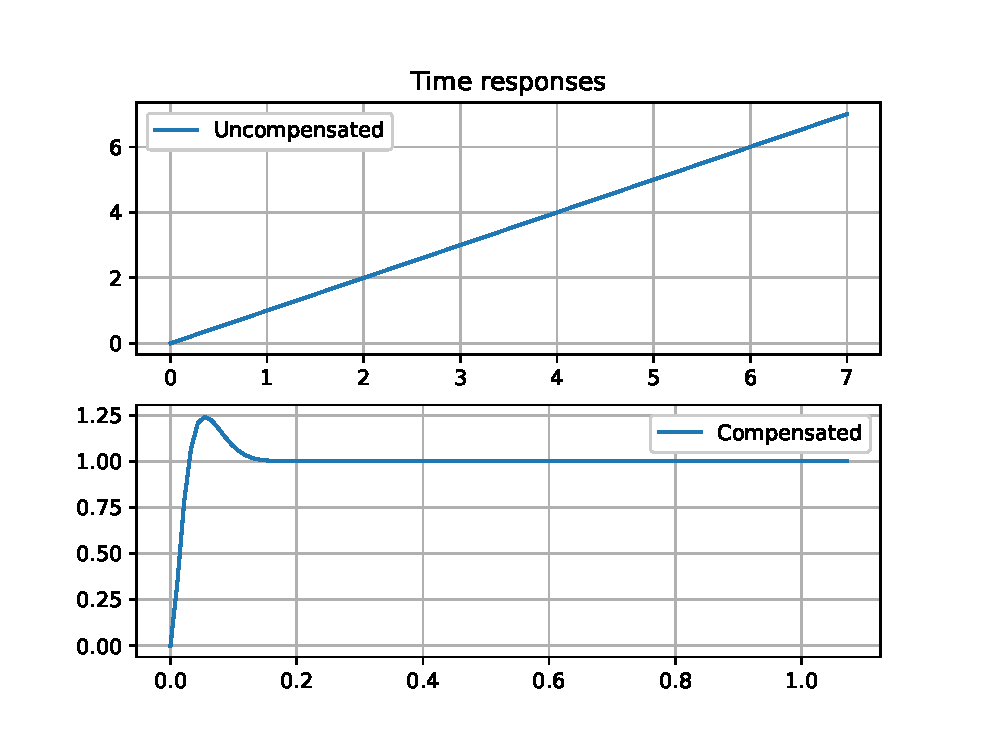
\includegraphics[width=\columnwidth]{./figs/ee18btech11012/ee18btech11012_3.eps}
\caption{}
\label{fig:ee18btech11012_4} 
\end{figure}
The following code can be verified
\begin{lstlisting}
codes/ee18btech11012/ee18btech11012_3.py
\end{lstlisting}
\item Verifying the designed lag-lead compensator \\
\solution 
\begin{table}[!ht]
\centering
\input{./tables/ee18btech11012/ee18btech11012_table1.tex}
\caption{Comparing the desired and obtained results}
\label{table:ee18btech11012_table1}
\end{table}
\end{enumerate}
}
\end{center}
\caption{}
\label{fig:ee18btech11012_1;}
\end{figure}
%
Velocity error constant  
\begin{align}
K_{v} &=  \lim_{s \to 0}sG(s)
\end{align}
\begin{align}
\lim_{s \to 0}s\frac{K(s+7)}{s(s+5)(s+15)} &= 1000
\end{align}
\begin{align}
\implies K &= 10714
\end{align}
Bode plot of G(s) for the value of K
%%
\begin{figure}[!ht]
\centering
  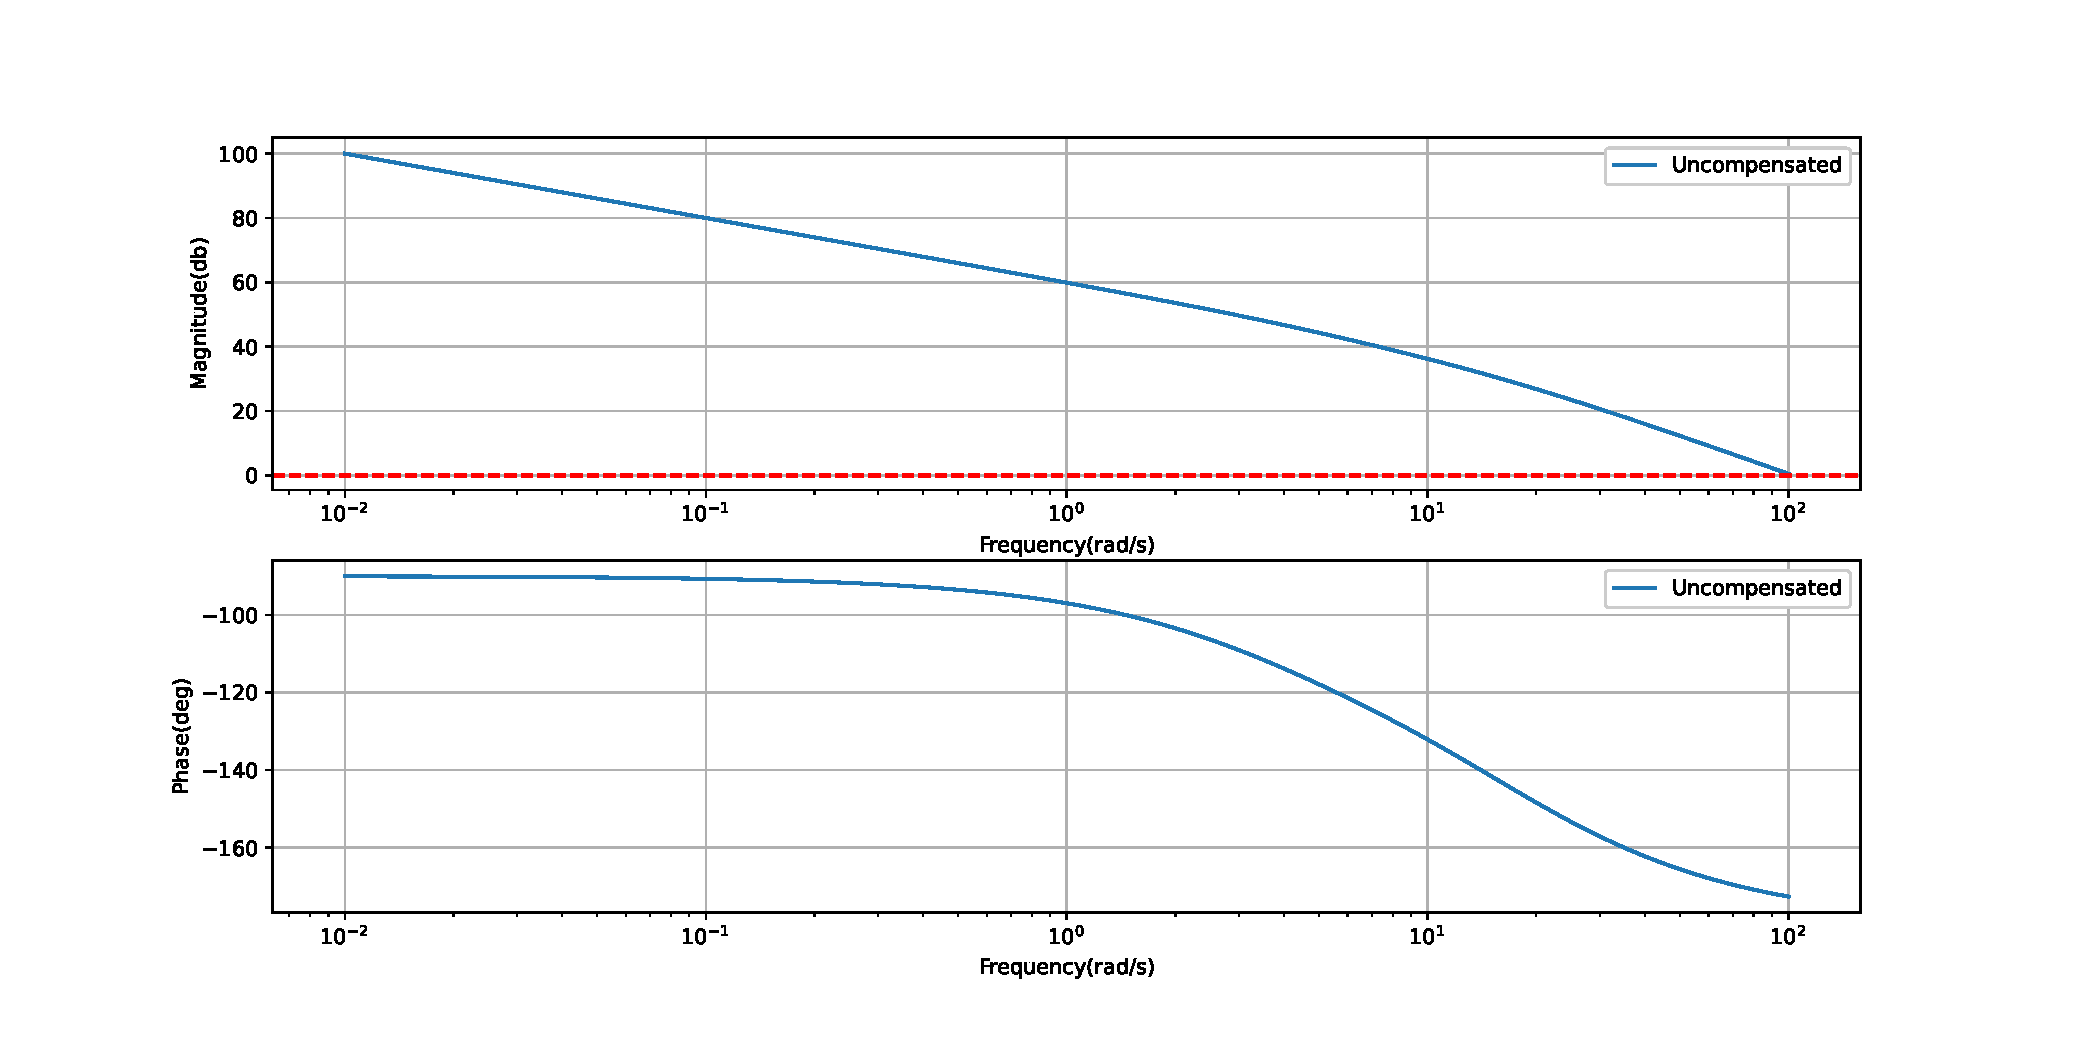
\includegraphics[width=\columnwidth]{./figs/ee18btech11012/ee18btech11012.eps}
\caption{}
\label{fig:ee18btech11012_2}
\end{figure}
%%
The following code verifies the result.
\begin{lstlisting}
codes/ee18btech11012/ee18btech11012_1.py
\end{lstlisting}
Relation between \%OS and Damping ratio
\begin{align}
\zeta &= \frac{-\ln(\%OS/100)}{\sqrt{(\pi)^2 + (\ln(\%OS/100))^2}}
\end{align}
\begin{align}
\implies\zeta &= 0.517 
\end{align}
Phase Margin for a Damping ratio is given by
\begin{align}
\phi_{m} &= 90\degree - \arctan(\frac{\sqrt{-2\zeta^2+\sqrt{1+4\zeta^4}}}{2\zeta}
\end{align}
\begin{align}
\implies \phi_{m} &= 53.17\degree
\end{align}
For an additional 5\degree for lag compensation,Phase margin is
\begin{align}
    \phi_{m} &= 53.17\degree + 5\degree= 58.17\degree
\end{align}
\textbf{Note} : Adding 5\degree phase angle to compensate the phase angle contribution of the lag compensator.
Bandwidth frequency is given by
\begin{align}
\omega_{BW} &= \omega_{n}(\sqrt{(1-2\zeta^2)+\sqrt{4\zeta^4-4\zeta^2+2}})
\end{align}
where
\begin{align}
    \omega_{n} &= \frac{4}{T_{s}\zeta}
\end{align}
Given settling time = 0.1 sec then 
\begin{align}
    \omega_{n} &= 77.37 rad/sec 
\end{align}
then
\begin{align}
    \omega_{BW} &= 96.91 rad/sec
\end{align}
\item Designing Lag-Lead Compensator Gc(s) \\
\solution 
General lag-lead compensator 
\begin{align}
G_{c}(s) &= \left(\frac{s+\frac{1}{T_1}}{s+\frac{\gamma}{T_1}}\right)\left(\frac{s+\frac{1}{T_2}}{s+\frac{1}{\gamma T_2}}\right) 
\end{align}
\begin{itemize}
\item Choose the new phase-margin frequency 
\begin{align}
    \omega_{Pm} &= 0.8 \omega_{BW} &= 77.53 rad/sec
\end{align}
\item At this phase-margin frequency,Phase angle is -170.52\degree.
\item Then the conribution required from the lead is
\begin{align}
    \phi_{max} &= 58.17-(180-170.52)=48.69\degree.
\end{align}

\item Now Using the relation 
\begin{align}
    \phi_{max} &= \sin^{-1}(\frac{1-\beta}{1+\beta})
\end{align}
then we get
\begin{align}
    \beta &= 0.142
\end{align}
\item \underline{Lag Compensator Design}:The Compensator must have a dc gain of unity to retain the value of Kv that we have already designed by setting K = 10714.
\begin{align}
    z_{clag} &= \frac{\omega_{Pm}}{10}=\frac{77.53}{10}=7.753
\end{align}
\begin{align}
    p_{clag} &= z_{clag}*\beta=1.102
\end{align}
Gain in the lag compensator is 
\begin{align}
    K_{clag} &= \frac{p_{clag}}{z_{clag}}=0.1421
\end{align}
\item Hence the lag compensator transfer function is
\begin{align}
 G_{clag}(s) &= \frac{0.1421(s+7.753)}{s+1.102} 
\end{align}
\item \underline{Lead Compensator Design}:DC gain for this must be unity.

\textbf{Relations to find T and $\beta$}:
The Compensator's magnitude at the phase margin frequency $\omega_{max}$
\begin{align}
     |G_{c}(j\omega_{max})| &= \frac{1}{\sqrt{\beta}} 
\end{align}
\begin{align}
    T &= \frac{1}{\omega_{max}\sqrt{\beta}}
\end{align}
So,To find transfer function
\begin{align}
    z_{lead} &= \frac{1}{T_{2}}=\omega_{Pm}*\sqrt{\beta}=29.92
\end{align}
\begin{align}
    p_{lead} &= \frac{z_{lead}}{\beta}=205.74,K_{lead}=\frac{p_{lead}}{z_{lead}}=7.04
\end{align}
\item Thus lead compensator transfer function is 
\begin{align}
    G_{lead} &= \frac{7.04(s+29.22)}{s+205.74} 
\end{align}
\item So the overall compensator tranfer function is
\begin{align}
    G_{c}(s) &= G_{clag}(s)G_{lead}(s)
\end{align}
\begin{align}
G_{c}(s)&=\frac{1.000384(s+7.753)(s+29.23)}{(s+1.102)(s+205.7)}
\end{align}
\end{itemize}
\item Verifying Lag-lead Compensator using Plots \\
\solution 
Magnitude and Phase plot
\begin{figure}[!ht]
\centering
  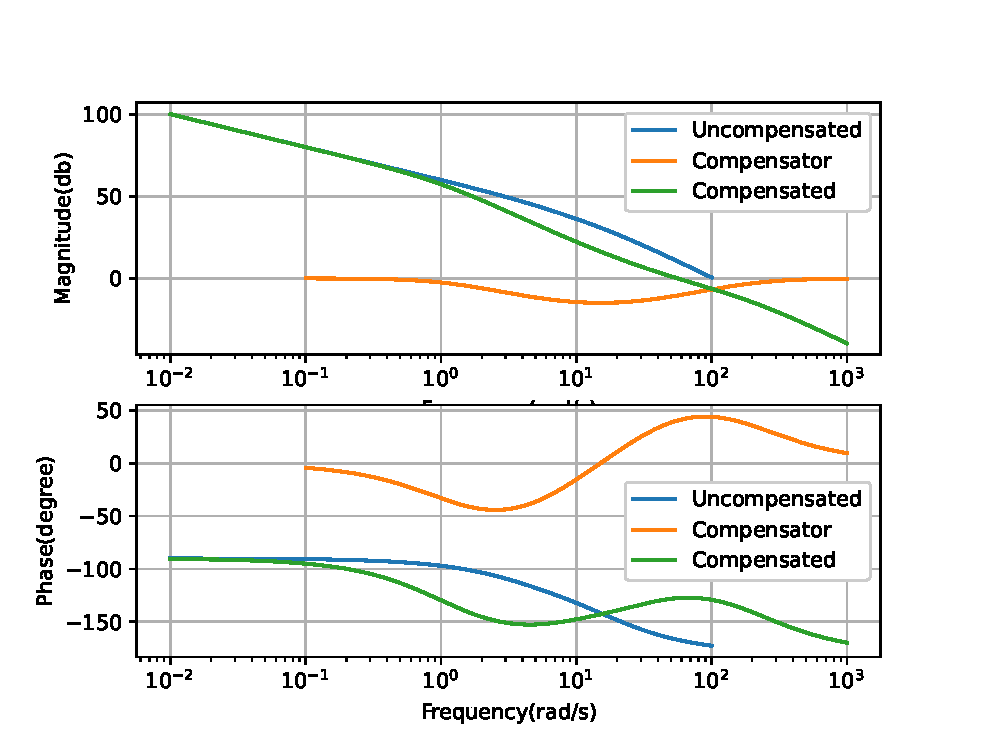
\includegraphics[width=\columnwidth]{./figs/ee18btech11012/ee18btech11012_2.eps}
\caption{}
\label{fig:ee18btech11012_3}
\end{figure}
The following code 
\begin{lstlisting}
codes/ee18btech11012/ee18btech11012_2.py
\end{lstlisting}
\item Verifying in time domain \\
\solution 
Time response for a unit step function
\begin{figure}[!ht]
\centering
  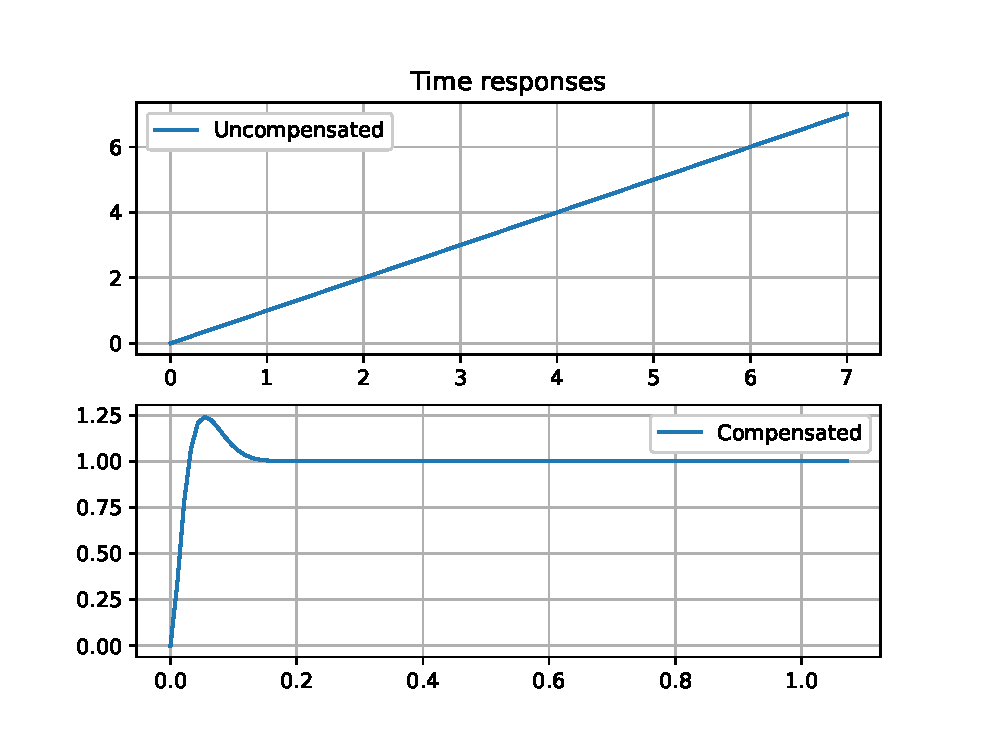
\includegraphics[width=\columnwidth]{./figs/ee18btech11012/ee18btech11012_3.eps}
\caption{}
\label{fig:ee18btech11012_4} 
\end{figure}
The following code can be verified
\begin{lstlisting}
codes/ee18btech11012/ee18btech11012_3.py
\end{lstlisting}
\item Verifying the designed lag-lead compensator \\
\solution 
\begin{table}[!ht]
\centering
\input{./tables/ee18btech11012/ee18btech11012_table1.tex}
\caption{Comparing the desired and obtained results}
\label{table:ee18btech11012_table1}
\end{table}
\end{enumerate}
